\documentclass{article}
\usepackage[utf8]{inputenc}

\title{GDD-TANKTALE}
\author{Damian Tomczyszyn}
\date{Październik 2020}

\usepackage{natbib}
\usepackage{graphicx}
\usepackage{polski}
\begin{document}

\maketitle

\centering
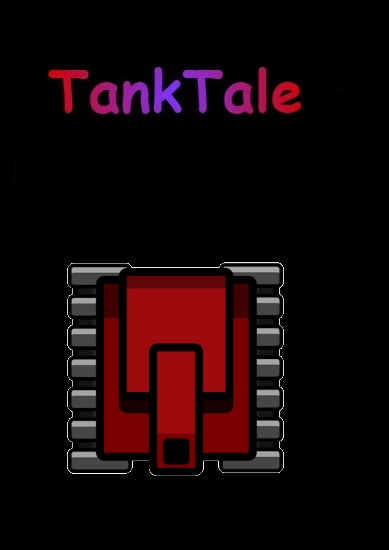
\includegraphics[scale=0.6,]{TT-logo.jpg}

\newpage
\centering	{Spis treści}
\begin{enumerate}
	\item Wprowadzenie
	    \item[*] Przyjęte konwencje
	    \item[*] Rejestr zmian
	\item Informacje ogólne
	    \item[*] Ogólny opis gry
	    \item[*] Motywacja i inspiracje
	    \item[*] Platformy docelowe
	    \item[*] Odbiorcy docelowi
	    \item[*] Decyzje technologiczne
	       \begin{enumerate}
	    \item[*] Silnik gry
	    \end{enumerate}
	    \item[*] Wykorzystywane licencje
	    \item[*] Język gry
	\item Tryby
	    \item[*] Tryb Kampani
	    \item[*] Tryb Przetrwania
    \item Interfejs użytkownika
        \item[*] Obsługa gry
	    \item[*] HUD
	    \item[*] Praca kamery
	    
	\item Mechanika Podstawowa
	    \item[*] Personifikacja gracza
	    \item[*] Plansza
	    \item[*] Poruszanie się
	    \item[*] Obiekty statyczne 
	    
	    \item[*] Obiekty dynamiczne 
	    
	    \item[*] Warunki ukończenia gry 
	    \begin{enumerate}
	    \item[*] Warunki dodatkowe
	    \end{enumerate}
	    
	    \item[*] Decyzje technologiczne
	    \item[*] Wykorzystywane licencje
	    \item[*] Język gry
	    
	\item Świat przedstawiony   
	    \item[*] Realia świata  
	    \item[*] Tło fabularne 
	    \item[*] Dzwięki i muzyka
        \item[*] Styl graficzny
	    \item[*] Waluta i surowce
	    
	    
	    
    \item  Inne tryby rozgrywki 
        \item[*] Wprowadzenie
	    \item[*] Tryby związane z menu głównym 
	    \item[*] Tryby związane z rozgrywką 

	\item  Informacje dodatkowe
	   
	\end{enumerate}
	
	
	
	
	
	\newpage
	
	
	
	
\section{Wprowadzenie}
    \subsection{Przyjęte konwencje}
\begin{itemize}
    \item Tekst napisany \emph{kursywą} dotyczy nazw własnych występujących w otocze-niu „zwykłego” tekstu oraz nazwy tej gry. Jest również wykorzystywanydo zaznaczenia używanych obcojęzycznych zwrotów lub nazw atrybutów.
\end{itemize}
    \subsection{Rejestr zmian}
\begin{tabular}{|l|c|r|}
	\hline
	Data Modyfikacji & Osoba & Komentarz\\
	\hline
	15.10.2020 & Damian Tomczyszyn & Utworzenie struktury dokumentu\\
	\hline
	31.10.2020 & Damian Tomczyszyn & Stworzenie spisu treści \\
	\hline
\end{tabular}

\newpage

\section{Informacje ogólne}
    \subsection{Ogólny opis gry}
    \emph{TANKTALE} jest grą RPG o tematyce rozwoju bohatera(czołgu z załogą). Gra jest przeznaczona dla jednego gracza, w której celem rozgrywki jest rozwijanie swojego pojazdu. Akcja gry rozgrywa się w świecie zniszczonym przez wojnę nuklearną. Sterujemy czołgiem który wyposarzony jest w działo, które jest główną bronią która pomaga pokonać przeciwników.Sama  idea  gry  topowrót do mechanizmów znanych ze starszych, grywalnych, prostych gier z po-wiewem świeżości w postaci większego systemu ulepszeń. Pojazd(bohater) musi oczyszyczszać strefy zwane \emph{hangarami} które po oczyszczeniu stają się bezpieczną zoną w której można handlować(kupować/sprzedawać przedmioty), dokonywać ulepszeń pojazdu, rozwijać umiejętności załogi oraz przeczekać do konkretnej godziny(możliwość szybkiej zmiany dnia na noc i na odwrót). 
    
    \subsection{Motywacja i inspiracje}
    \begin{itemize}
        \item Tytułem inspirowałem się na grze która mnie mocno poruszyła- UnderTale.
        \item Czas rozgrywania się akcji, oraz niektórzy przeciwnicy to pomysł pożyczony z serii Metro.
    \end{itemize}
    \subsection{Platformy docelowe}
    Platformą docelową gry są komputery stacjonarne wyposażone w system Windows.
    \subsection{Odbiorcy docelowi}
    Odbiorcami docelowymi są zarówno dorośli jak i młodzi gracze.
    \subsection{Decyzje technologiczne}
    \begin{enumerate}
       \item C sharp - Język w którym gra jest tworzona
    \item Sterowanie za pomocą "WASD" oraz myszki
     \item Możliwość obrotu kamery strzałkami
     \item Konieczne  jest  stworzenie  rysunkowego  i  estetycznego  stylu  graficznego,aby gra zachęcała odbiorców warstwą wizualną \item Silnik Godot
\end{enumerate}

\subsection{Wykorzystane licencje}
Do  realizacji  gry  nie  będzie  konieczne  nabycie  żadnych  licencji  związanych  zpodjętymi decyzjami technologicznymi, gdyż przyjęte środowisko ma charakterotwarty i darmowy. Nie ma również potrzeby starania się o kupno licencji zwią-zanych ze światem gry lub patentami, gdyż małe fragmenty świata fabularnegogry  są  stworzone  całkowicie  przez  autorów,  natomiast  mechanika  podobnychgier nie jest objęta ochroną prawną
\newpage

\section{Tryby}
    \subsection{Tryb kampani}
Podstawowym trybem gry \emph{TANKTALE} jest forma kampanii. Gracz rozpoczyna swoją przygodę z grą od pierwszej planszy w obrębie danej grupy, a następnie po jej ukończeniu ma dostęp do kolejnej mapy.
    \subsection{Tryb Przetrwania}
Innym trybem gry jest tryb przetrwania \emph{(survival mode)}. Gracz rozpoczyna grę z wybranym wyposarzeniem na otwartej mapie i jego zadaniem jest pokonanie jak największej liczby przeciwników - uzyskanie jak największego wyniku(przetrwany czas + punkty za zabite potwory).
    \newpage
    
\section{Interfejs użytkownika}
    \subsection{Obsługa gry}
Gra \emph{TANKTALE} jest zaprojektowana na urządzenia posiadajace klawiaturę oraz mysz. Więc sterowanie jest dość proste:
\begin{itemize}
    \item Klawisze WASD - poruszanie się pojazdu.
    \item Mysz- poruszanie się kamery, celowanie(ppm) , oddawanie strzału(lpm).
    \item Klawisz R - ładowanie
    \item strzałki - poruszanie się kamerą.
    \item shift - zmniejszenie możliwości wykrycia
    \item crtl + ppm - badanie celu (hp przeciwnika)
    \item tab Przełączanie pomiędzy załogą w celu uzyskania dokładniejszych informacji
    \item 1,2,3,4,5 zmiana rodzaju amunicji
    
\end{itemize}
    \subsection{HUD}
    \subsection{Praca kamery}
    Plansza  wraz  z  wszystkimi  elementami  ukazywana  jest  w  dwóch  wymiarach,jako  widok  z  góry,  podobny  do  tego  znanego  z  gierDyna  BlasterczyPac-Man.
    \newpage
    
\section{Mechanika podstawowa}
    \subsection{Personifikacja gracza}
    Gracz steruje bohaterem(pojazdem-czołgiem) przemierzającym świat i starajacym się oczyszczać teren.
    \subsection{Plansza}
    Rozgrywka toczy się na pewnej planszy. Jak wspominano wcześniej jest to powojenny świat z dominującą pustynną tematyką. Można w nim będzie spotka wiele wraków pojazdów oraz zniszczone i opuszczone miasta.
    \subsection{Poruszanie się}
    Gracz może poruszać się WASD(nie podczas interakcji).
    \subsection{Obiekty statyczne}
    \begin{itemize}
        \item Budynki
        \item Wraki
        \item Mosty
        \item Skały
        \item Hangary
        
    \end{itemize}
    \subsection{Obiekty dynamiczne}
    \begin{itemize}
        \item przeciwnicy
        \begin{enumerate}
            \item Trigeny/mutanty
            \item Drzewce
            \item Inne czołgi
        \end{enumerate}
        \item sojusznicze czołgi
        \item Zaopatrzeniowcy
        \item Nietoperze
        \item Pająki
        \item Pułapki
        
    \end{itemize}
    \subsection{Warunki ukończenia gry}
\begin{itemize}
    \item Wygrana
    \begin{enumerate}
        \item Zabicie wszystkich przeciwników.
        \item Wykonanie wszystkich questów.
        \item Przejęcie wszystkich \emph{hangarów}.
    \end{enumerate}
    \item Przegrana
    \begin{enumerate}
        \item Strata całego HP.
        \item Strata paliwa i brak możliwości wezwania zrzutu zaopatrzenia
    \end{enumerate}
\end{itemize}
    
    \newpage
    
   
\section{Świat przedstawiony}
    \subsection{Realia świata}
    \begin{itemize}
 

    \item Świat w grze jest wyniszczony wojną nuklearną. Większość obszarów stanowi pustynia. Od czasu do czasu występują zniszczone miasta i wraki różnych pojazdów. Teren nie jest mocno górzysty, ale występują wertepy i wysepki. Całą planszę otaczają skały nie pozwalające wypaść poza mapę. 
\item Hangary - są miejscem w którym można przespać się(zmienić godzinę i porę dnia). Można handlować, naprawiać pojazd, ulepszać pojazd, rozdawać umiejętności. Hangar będzie miejscem po którym nie można się poruszać. Będzie obrazkiem na którym można wybrać interesujące nas opcje(handlu/snu/umiejętności/zapisu gry).
    \end{itemize}
    \subsection{Tło fabularne}
    Historia w grze na starcie opowiada: 
    \begin{enumerate}
        \item Jak doszło do wojny
        \item Skąd wzięły się czołgi i hangary
        \item Jaka jest waluta i co jest ważne w tym świecie
        \item Jak powstały mutanty
        \item I jak to jest z nacjami
        \item Oraz wprowadza gracza w pierwsze zadanie i samouczek
    \end{enumerate}
    \subsection{Dzwięki i muzyka}
    
    
    \subsection{Styl graficzny}
    
    
    \subsection{Waluta i surowce}
    \begin{enumerate}
        \item Paliwo
        \item Złom(waluta)
    \end{enumerate}
    \newpage
    
\section{Inne tryby rozgrywki}
    \subsection{Wprowadzenie}
    W poniższym rozdziale opisane są zidentyfikowane tryby rozgrywki z pominię-ciem głównego trybu (samej rozgrywki), na który przeznaczona została więk-szość poprzednich rozdziałów.
    
    \subsection{Tryby związane z menu głównym}
    \begin{enumerate}
        \item ekran powitalny
        Ekran powitalny jest wczytywany i uruchamiany od razu po uruchomieniu apli-kacji. Jego przeznaczeniem jest poinformowanie gracza o włączanej aplikacji iwprowadzenie w klimat gry. W trakcie wyświetlania ekranu powitalnego łado-wane są zasoby gry – w związku z tym, na ekranie jest wyświetlana informacjao procesie ładowania, a po jego zakończeniu pojawia się informacja zachęcającaużytkownika do dotknięcia kliknięcia 'Enter' i przejścia do menu głównego.
        \item Menu główne
        Menu główne jest jednym z dwóch głównych trybów rozgrywki, któremu podle-gają inne ekrany i jest uruchamiane po ekranie powitalnym. Umożliwia m.in. pod-jęcie rozgrywki (ostatniej lub na jednym z wcześniej odkrytych poziomów), zmia-nę  ustawień  gry,  odwiedzenie  sklepu  i  przeglądnięcie  innych  informacji. 
        \item Osiągnięcia
        \item Ustawienia gry
        \begin{itemize}
            \item zmiana głośności muzyki
            \item zmiana głoścności efektów dzwiękowych
            \item Zmmiana ogólnej głośności gry
        \end{itemize}
        
    \end{enumerate}
    
    \subsection{Tryby związane z rozgrywką}
    \begin{enumerate}
        \item Ekran informacji o poziomie
        \item Rozgrywka
        \item Ekran końca planszy
        
    \end{enumerate}
        
    
    
    \newpage
    
\section{Informacje dodatkowe}



\end{document}
